 
\section{\ix Implementation}
\label{sec:impl}

\begin{table*}[t]
\centering
\begin{small}
\begin{tabular}{|l|l|l|}
\hline
\multicolumn{3}{|c|}{{\bf System Calls (batched)}} \\
\hline
connect &             cookie, dst\_IP, dst\_port		& Opens a connection\\
accept &              handle, cookie				& Accepts a connection\\
sendv &               handle, scatter\_gather\_array		& Transmits a scatter-gather array of data\\
recv\_done &          handle, bytes\_acked			& Advances the receive window and frees memory buffers\\
close &               handle					& Closes or rejects a connection\\
\hline  \hline
\multicolumn{3}{|c|}{{\bf Event Conditions}} \\
\hline
{\bf Type} &           {\bf Parameters}  &
{\bf Description}\\
knock  &               handle, src\_IP, src\_port		& A remotely initiated connection was opened \\
connected &            cookie, outcome				& A locally initiated connection finished opening \\
recv &                 cookie, mbuf\_ptr, mbuf\_len		& A message buffer was received \\
sent &                 cookie, bytes\_sent, window\_size	& A send completed and/or the window size changed \\
dead &                 cookie, reason				& A connection was terminated \\
\hline
\end{tabular}
\caption{\ix system calls and event conditions API. 
}
\label{tbl:api}
\end{small}
\end{table*}



% \christos{We should stress that the same pattern/architecture can be
%   used to implement any high performance stack, not just TCP/IP}


\subsection{Overview}
\label{sec:impl:overview}

Fig.~\ref{fig:cp-dp} presents the \ix architecture, focusing on the
separation between the control plane and the multiple dataplanes.  The
hardware environment is a multi-core server with one or more
multi-queue NICs with RSS support. The \ix control plane consists of the full Linux kernel and
\texttt{IXCP}, a user-level program. The Linux kernel
initializes PCIe devices, such as the NICs, and provides the basic
mechanisms for resource allocation to the dataplanes, including cores,
memory, and network queues. Equally important, Linux provides system
calls and services that are necessary for compatibility with a wide
range of applications, such as file system and signal
support. \texttt{IXCP} monitors resource usage and dataplane
performance and implements resource allocation policies. The
development of efficient allocation policies involves understanding
difficult tradeoffs between dataplane performance, energy
proportionality, and resource sharing between co-located applications
as their load varies over time. We leave the design of such policies
to future work and focus primarily on the \ix dataplane architecture.

We run the Linux kernel in VMX root ring 0, the mode typically used to
run hypervisors in virtualized
systems~\cite{DBLP:journals/computer/UhligNRSMABKLS05}. We use the
Dune module within Linux to enable dataplanes to run as
application-specific OSes in the VMX non-root ring 0, the mode
typically used to run guest kernels in virtualized
systems~\cite{dune}.  Applications run in VMX non-root ring 3, as
usual.  This approach provides dataplanes with direct access to
hardware features, such as page tables and exceptions, and pass-through
access to NICs. Moreover, it provides full, three-way protection
between the control plane, dataplanes, and untrusted application code.

Each \ix dataplane supports a single, multithreaded application. For
instance, Fig.~\ref{fig:cp-dp} shows one dataplane for a
multi-threaded \texttt{memcache} server and another dataplane for a
multi-threaded \texttt{http} server. The control plane allocates
resources to each dataplane in a coarse-grained manner. Core
allocation is controlled through real-time priorities and
\texttt{cpusets}; memory is allocated in large pages; each NIC
hardware queue is assigned to a single dataplane. This approach avoids
the overheads and unpredictability of fine-grained time multiplexing
of resources between demanding
applications~\cite{DBLP:conf/eurosys/LeverichK14}.

The \ix dataplane operates as a single address-space OS and supports
two thread types within the shared, user-level address space: (i)
\emph{elastic threads} which interact with the \ix dataplane to
initiate and consume network I/O and (ii) \emph{background threads}.
Both elastic and background threads can issue arbitrary POSIX system
calls that are intermediated and validated for security by the
dataplane before being forwarded to the Linux kernel. Elastic threads
are expected to \emph{not} issue blocking calls because of the adverse
impact on network behavior and performance. Similarly, each elastic
thread makes exclusive use of a core or hardware thread allocated to
the dataplane in order to achieve high performance with predictable
latency. In contrast, multiple background threads may timeshare an
allocated hardware thread. For example, if an application were
allocated four hardware threads, it could use all of them as elastic
threads to serve external requests or it could temporarily transition
to three elastic threads and use one background thread to execute
tasks such as garbage collection. When the control plane revokes or
allocates an additional hardware thread using a protocol similar to
the one in Exokernel~\cite{DBLP:conf/sosp/EnglerKO95}, the dataplane
adjusts its number of elastic threads.

% \christos{We should stress that queues are a central concept in our
%   work.  we should add some discussion about elasticity/load balancing
%   here. Should we discuss how traffic is seperated between queues in
%   this section?}

\subsection{The \ix Dataplane}
\label{sec:impl:dpkernel}

We now discuss the \ix dataplane in more detail. It differs from a typical
kernel in that it is specialized for high performance I/O and runs only a single
application, similar to a library OS but with memory
isolation. However, our dataplane still provides many
familiar kernel-level services.

For memory management, we accept some memory fragmentation in order to
reduce complexity and improve efficiency. All hot-path data objects
are allocated from per hardware thread memory pools. Each memory pool
is structured as arrays of identically sized objects, provisioned in
page-sized blocks. Free objects are tracked with a simple free list,
and allocation routines are inlined directly into calling
functions. \emph{Mbufs}, the storage object for network packets, are stored
as contiguous chunks of bookkeeping data and MTU-sized buffers, and
are used for both receiving and transmitting packets.

The dataplane also manages its own virtual address translations,
supported through nested paging. In contrast to contemporary OSes, it
uses exclusively large pages (2MB). We favor large pages due to
their reduced address translation
overhead~\cite{DBLP:conf/isca/BasuGCHS13, dune} and the relative
abundance of physical memory resources in modern servers. The
dataplane maintains only a single address space; kernel pages are
protected with supervisor bits. We deliberately chose not to support
swappable memory in order to avoid adding performance variability.

We provide a hierarchical timing wheel implementation for managing
network timeouts, such as TCP
retransmissions~\cite{DBLP:conf/sosp/VargheseL87}. It is optimized for
the common case where most timers are canceled before they expire. We
support extremely high resolution timeouts, as low as 16 \microsecond,
which has been shown to improve performance during TCP incast
congestion~\cite{DBLP:conf/sigcomm/VasudevanPSKAGGM09}.

Our current \ix dataplane implementation (and Dune) requires
the VT-x virtualization features available on Intel x86-64
systems~\cite{DBLP:journals/computer/UhligNRSMABKLS05}. However, it
could be ported to any architecture with virtualization support, such as
ARM, SPARC, and Power. It also requires one or more Intel 82599 chipset NICs,
but it is designed to easily support additional drivers.
Moreover, the \ix dataplane currently consists of 39K
SLOC~\cite{url:sloccount} and leverages some existing codebases:
41\% is derived from
the DPDK variant of the Intel NIC device driver~\cite{intel:dpdk},
26\% from the lwIP TCP/IP stack~\cite{dunkels2001design},
and 15\% from the Dune library.  We do not make use of the DPDK
framework, and all three code bases are
highly modified for \ix. The rest is approximately 7K SLOC
of new code. We chose lwIP as a starting point for TCP/IP processing
because of its modularity and its maturity as a RFC-compliant,
feature-rich networking stack. We implemented RFC-compliant support
for UDP, ARP, and ICMP.  Since lwIP was optimized for memory
efficiency in embedded environments, we had to radically change its
internal data structures for multi-core scalability and fine-grained
timer management. However, we did not yet optimize the lwIP code for
performance. Hence, there is room for improvement in the results shown
in \S\ref{sec:eval}.

\subsection{Dataplane API and Operation}
\label{sec:impl:api}

Elastic threads interact with the \ix dataplane through three
asynchronous, non-blocking mechanisms summarized in
Table~\ref{tbl:api}: they issue \emph{batched systems calls} to the
dataplane; they consume \emph{event conditions} generated by the
dataplane; and they have direct, but safe, access to (\emph{mbuf}s)
containing incoming payloads.  The latter allows for zero-copy access
to incoming network traffic.  The application can hold on to mbufs
until it asks the dataplane to release them via the
\texttt{recv\_done} batched system call.

Both batched system calls and event conditions are passed through
arrays of shared memory, managed by the user and the kernel
respectively.  \ix provides an unbatched system call
(\texttt{run\_io}) that yields control to the kernel and initiates a
new run to completion cycle. As part of the cycle, the kernel
overwrites the array of batched system call requests with
corresponding return codes and populates the array of event
conditions.  The handles defined in Table~\ref{tbl:api} are
kernel-level flow identifiers. Each handle is associated with a
cookie, an opaque value provided by the user at connection
establishment to enable efficient user-level state
lookup~\cite{DBLP:conf/osdi/HanMCR12}. %without an additional table lookup.

\ix differs from POSIX sockets in that it directly exposes flow
control conditions to the application. The \texttt{sendv} system call
does not return the number of bytes buffered. Instead, it returns the
number of bytes that were accepted and sent by the TCP stack, as
constrained by correct TCP sliding window operation. When the receiver
acknowledges the bytes, a \texttt{sent} event condition informs the
application that it is possible to send more data. Thus, send window
sizing policy is determined entirely by the application.  By contrast,
conventional OSes buffer send data beyond raw TCP constraints and
apply flow control policy inside the kernel.

%One hazard of working with batched system calls is that when one
%request depends on the outcome of another request in the batch, it can
%lead to unexpected results. For example, when two separate write
%requests are made to the same TCP connection, the first could fail,
%perhaps the kernel ran out of memory, while the second could succeed,
%resulting in incorrect ordering in the socket data stream. While not
%always required, we found that the simple heuristic of issuing at most
%one system call per TCP connection in a given batch greatly simplified
%error handling. The \texttt{sendv} system call also supports multiple
%buffers, so it is usually possible to coalesce several writes into a
%single request.

We built a user-level library, called \emph{libix}, which abstracts
away the complexity of our low-level API. It provides a compatible
programming model for legacy applications and significantly simplifies
the development of new applications. Libix currently includes a
functionally compatible interface to \texttt{libevent} and
non-blocking POSIX socket operations. It also includes new interfaces
for zero copy read and write operations that are more efficient, at
the expense of requiring changes to existing applications.

Libix automatically coalesces multiple write requests into single
\texttt{sendv} system calls during each batching round. This improves
locality, simplifies error handling, and ensures correct behavior,
as it preserves the data stream order even if a transmit fails.
Coalescing also facilitates transmit flow control because
we can use the transmit vector (the argument to \texttt{sendv})
to keep track of outgoing data buffers and, if necessary, reissue
writes when the transmit window has more available space, as notified
by the \texttt{sent} event condition. Our buffer sizing policy is currently
very basic; we enforce a maximum pending send byte limit, but
we plan to make this more dynamic in the future~\cite{dynamicwindow}.


%\begin{figure}
%\hspace*{-0.25in}\centering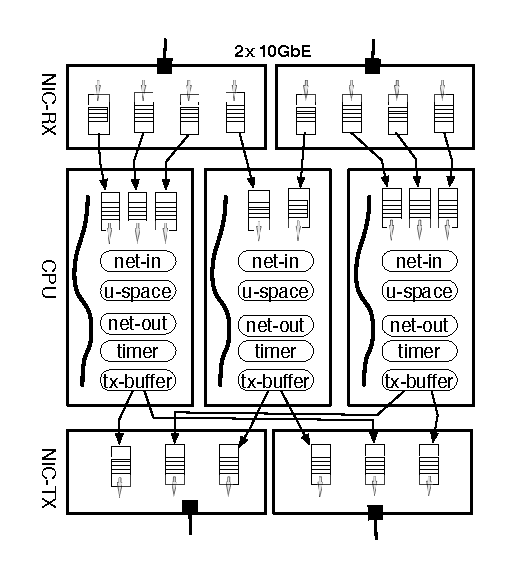
\includegraphics{figs/queues-cores.eps}
\centering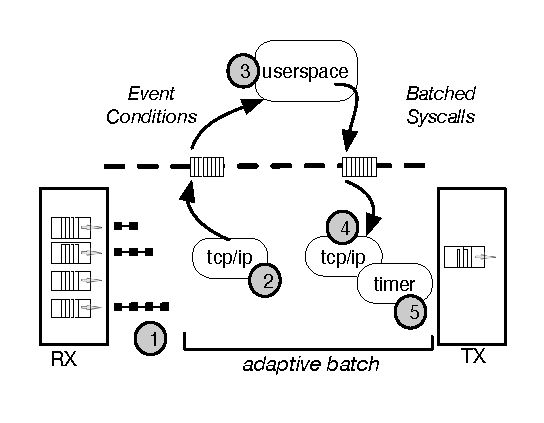
\includegraphics{figs/pipeline}
\caption{The IX pipeline.}
\label{fig:queues-cores}
\end{figure}

 

Fig.~\ref{fig:dataplane} illustrates the run-to-completion operation
for an elastic thread in the \ix dataplane. NIC receive buffers are
mapped in the server's main memory and the NIC's receive descriptor
ring is filled with a set of buffer descriptors that allow it to
transfer incoming packets using DMA\@.  The elastic thread (1) polls
the receive descriptor ring and potentially posts fresh buffer
descriptors to the NIC for use with future incoming packets. The
elastic thread then (2) processes a bounded number of packets through
the TCP/IP networking stack, thereby generating event
conditions. Next, the elastic thread (3) switches to the user-space
applications, which consumes all event conditions. Assuming that the
incoming packets include remote requests, the application processes
these requests and responds with a batch of system calls. Upon return
of control from user-space, the elastic thread (4) processes all batched
system calls, and in particular the ones that direct outgoing TCP/IP
traffic. It also (5) runs all kernel timers in order to ensure
compliant TCP behavior. Finally (6), it places outgoing Ethernet
frames in the NIC's transmit descriptor ring for transmission, and it
notifies the NIC to initiate a DMA transfer for these frames by
updating the transmit ring's tail register. In a separate pass, it
also frees any buffers that have finished transmitting, based oh the
transmit ring's head position, potentially generating \texttt{sent}
event conditions.  The process repeats in a loop until there is no
network activity. In this case, we enter a quiescent state which
involves either hyperthread-friendly polling or optionally entering a
power efficient C-state, at the cost of some additional latency.


\subsection{Multi-core Scalability}
\label{sec:impl:cohfree}

The \ix dataplane is optimized for multi-core scalability, as elastic
threads operate in a synchronization and coherence free manner in the
common case. This is a stronger requirement than lock-free
synchronization, which requires expensive atomic instructions even
when a single thread uses a particular data structure in the common
case~\cite{DBLP:conf/sosp/DavidGT13}.  This is made possible through a
set of conscious design and implementation tradeoffs.

First, system call implementations can only be synchronization-free if
the API itself is
commutative~\cite{DBLP:conf/sosp/ClementsKZMK13}. The \ix API is
commutative between elastic threads. Each elastic thread has its own
flow identifier namespace, and an elastic thread cannot directly perform
operations on flows that it does not own.
%Events are processed independently on each elastic
%thread. Handles identify flows but cannot be exchanged between elastic
%threads. There is no file descriptor namespace.

Second, the API implementation is carefully optimized.  Each elastic
thread manages its own memory pools, hardware queues, event condition
array, and batched system call array. The implementation of event conditions and
batched system calls benefits directly from the explicit, cooperative
control flow transfers between \ix and the application.% by the elastic thread.
Since there is no concurrent execution by producer and
consumer, event conditions and batched system calls are implemented
without synchronization primitives based on atomics.

Third, the use of flow-consistent hashing at the NICs ensures that
each elastic thread operates on a disjoint subset of incoming TCP
flows. Hence, no synchronization or coherence occurs during the
processing of incoming requests for a server application. For client
applications with outbound connections, we need to ensure that the
reply is assigned to the same elastic thread that made the
request. Since we cannot reverse the Toeplitz hash used by
RSS~\cite{url:rss}, we simply probe the ephemeral port range to find a
port number that would lead to the desired behavior. Note that this
implies that two elastic threads in a client cannot share a flow to a
server.

\ix does have a small number of shared structures, including some that
require synchronization on updates.  For example, the ARP table is
shared by all elastic threads and is protected by RCU
locks~\cite{mckenney1998read}. Hence, the common case reads are
coherence-free but the rare updates are not.
RCU objects are garbage collected after a quiescent period that
spans the time it takes each elastic thread to finish a run to
completion cycle.
%
%\dm{Can you add a sentence about what constitutes a quiescent period
%  for RCU garbage collection, given that this is a very non-Linux
%  API?}

\ix requires synchronization when the control plane reallocates
resources between dataplanes.  For instance, when a core is revoked
from a dataplane, the corresponding network flows must be assigned
to another elastic thread. Such events are rare because resource
allocation happens in a coarse-grain manner. Finally, the application
code may include inter-thread communication and synchronization. While
using \ix does not eliminate the need to develop scalable application
code, it ensures that there are no scaling bottlenecks in the system
and protocol processing code.

\subsection{Security Model}
\label{sec:impl:coop}

% \christos{We need to clean up this section, make a bigger deal out of
%   this, and explain why this is the right way to architect IO
%   stacks/libOS}

The \ix API and implementation has a cooperative flow control
model between application code and the network-processing stack.
Unlike user-level stacks that allow user code to control networking
behavior, the \ix protection model makes few assumptions about
application. A malicious or misbehaving application can only hurt
itself. It cannot corrupt the networking stack or affect other
applications. All application code in \ix runs in user-mode, while the
dataplane code is in protected ring 0. Applications cannot access
dataplane memory, except for read-only message buffers.  No sequence
of batched system calls or other user-level actions can be used to
violate correct adherence to TCP and other network specifications.
Furthermore, the dataplane can be used to enforce network security
policies (e.g., iptables or Amazon Security
Groups~\cite{url:amazon-sg}) or to implement the network
virtualization functions typically done in a
hypervisor~\cite{nsdi:nsx}. The \ix security model is as strong as
conventional kernel-based networking stacks, a feature that is missing
from all recently proposed user-level stacks.

The \ix dataplane and the application collaboratively manage
memory. To enable zero-copy operation, a buffer used for an incoming
packet is passed read-only to the application, enabling zero-copy
operation. Applications that hold on to message buffers for extensive
periods of time must bound their use of this shared resource.  In the
transmit direction, zero-copy operation implies that the application
must not modify outgoing data until reception is acknowledged by the
peer.

Since elastic threads in \ix execute both the network stack and
application code, a long running application can block further network
processing for a set of queues. This behavior in no way affects other
applications or dataplanes. We use a timeout interrupt to detect
elastic threads that spend excessive time in user mode (e.g., in
excess of 10ms). We mark such applications as non-responsive and
notify the control plane.

The \ix current implementation does not use an IOMMU due to its
performance overheads~\cite{iommu:overhead}. The \ix kernel is trusted
code that has access to descriptor rings with host-physical addresses.
This decision is not fundamental to our design and does not affect the
security model provided to applications.


%\dm{This raised a couple of questions for me.  First, is the
%  immutability of transmit buffers enforced by memory protection, or
%  just by convention.  In other words, can you cause TCP segments to
%  be sent with bad checksums or otherwise shoot yourself in the foot
%  by writing to buffers in the send queue?  Second, why are message
%  buffers read-only (or does this exclude the actual payload part).
%  For example, if I'm implementing an HTTP proxy, can I make small
%  modifications to a message buffer I just received and then
%  retransmit it?  Or is the point that one would use scatter gather IO
%  for such surgical edits?} \christos{add a comment someplace about
%  checksum in HW}

